\begin{figure}
\centering
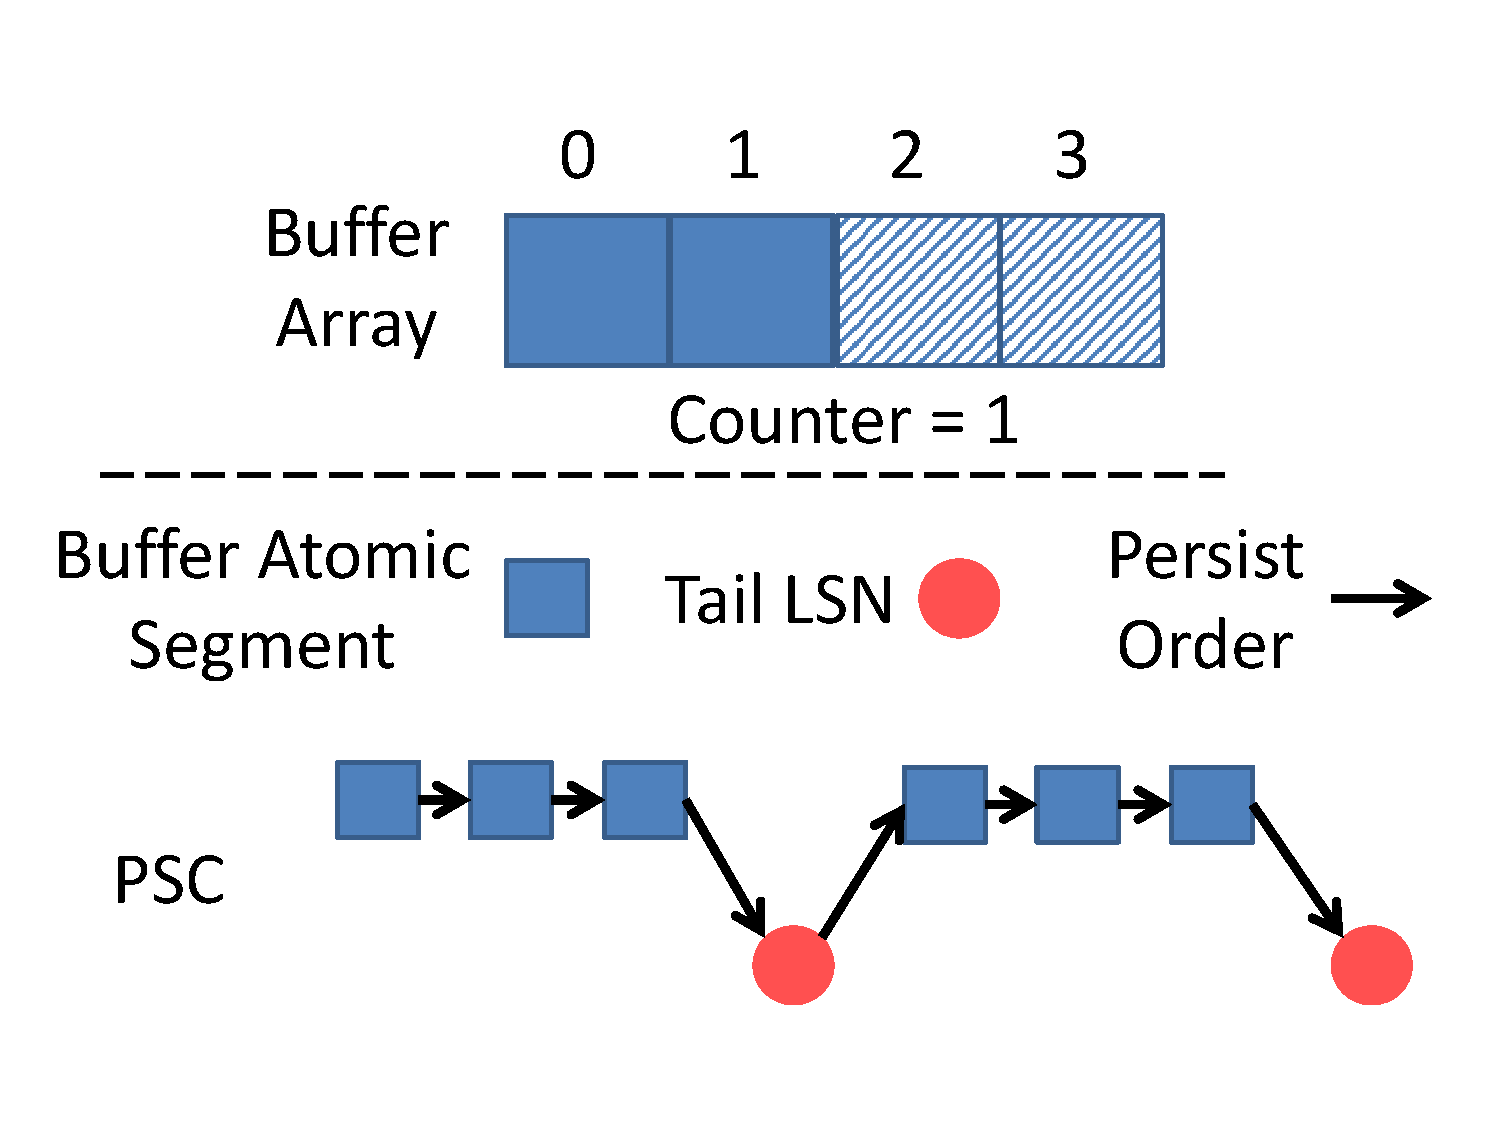
\includegraphics[width=.7\textwidth]{PMC_patterns/buffer.pdf}
\caption{\textbf{Persistent buffer.} The persistent buffer constists of a persistent array and counter (top).  The persistent counter marks the greatest persistent byte.  Persisting to the buffer under PSC places creates between writing buffer data and updating the counter, as well between persisting the counter and the next buffer persist, forming a chain (bottom).}
\label{fig:buffer}
\end{figure}
